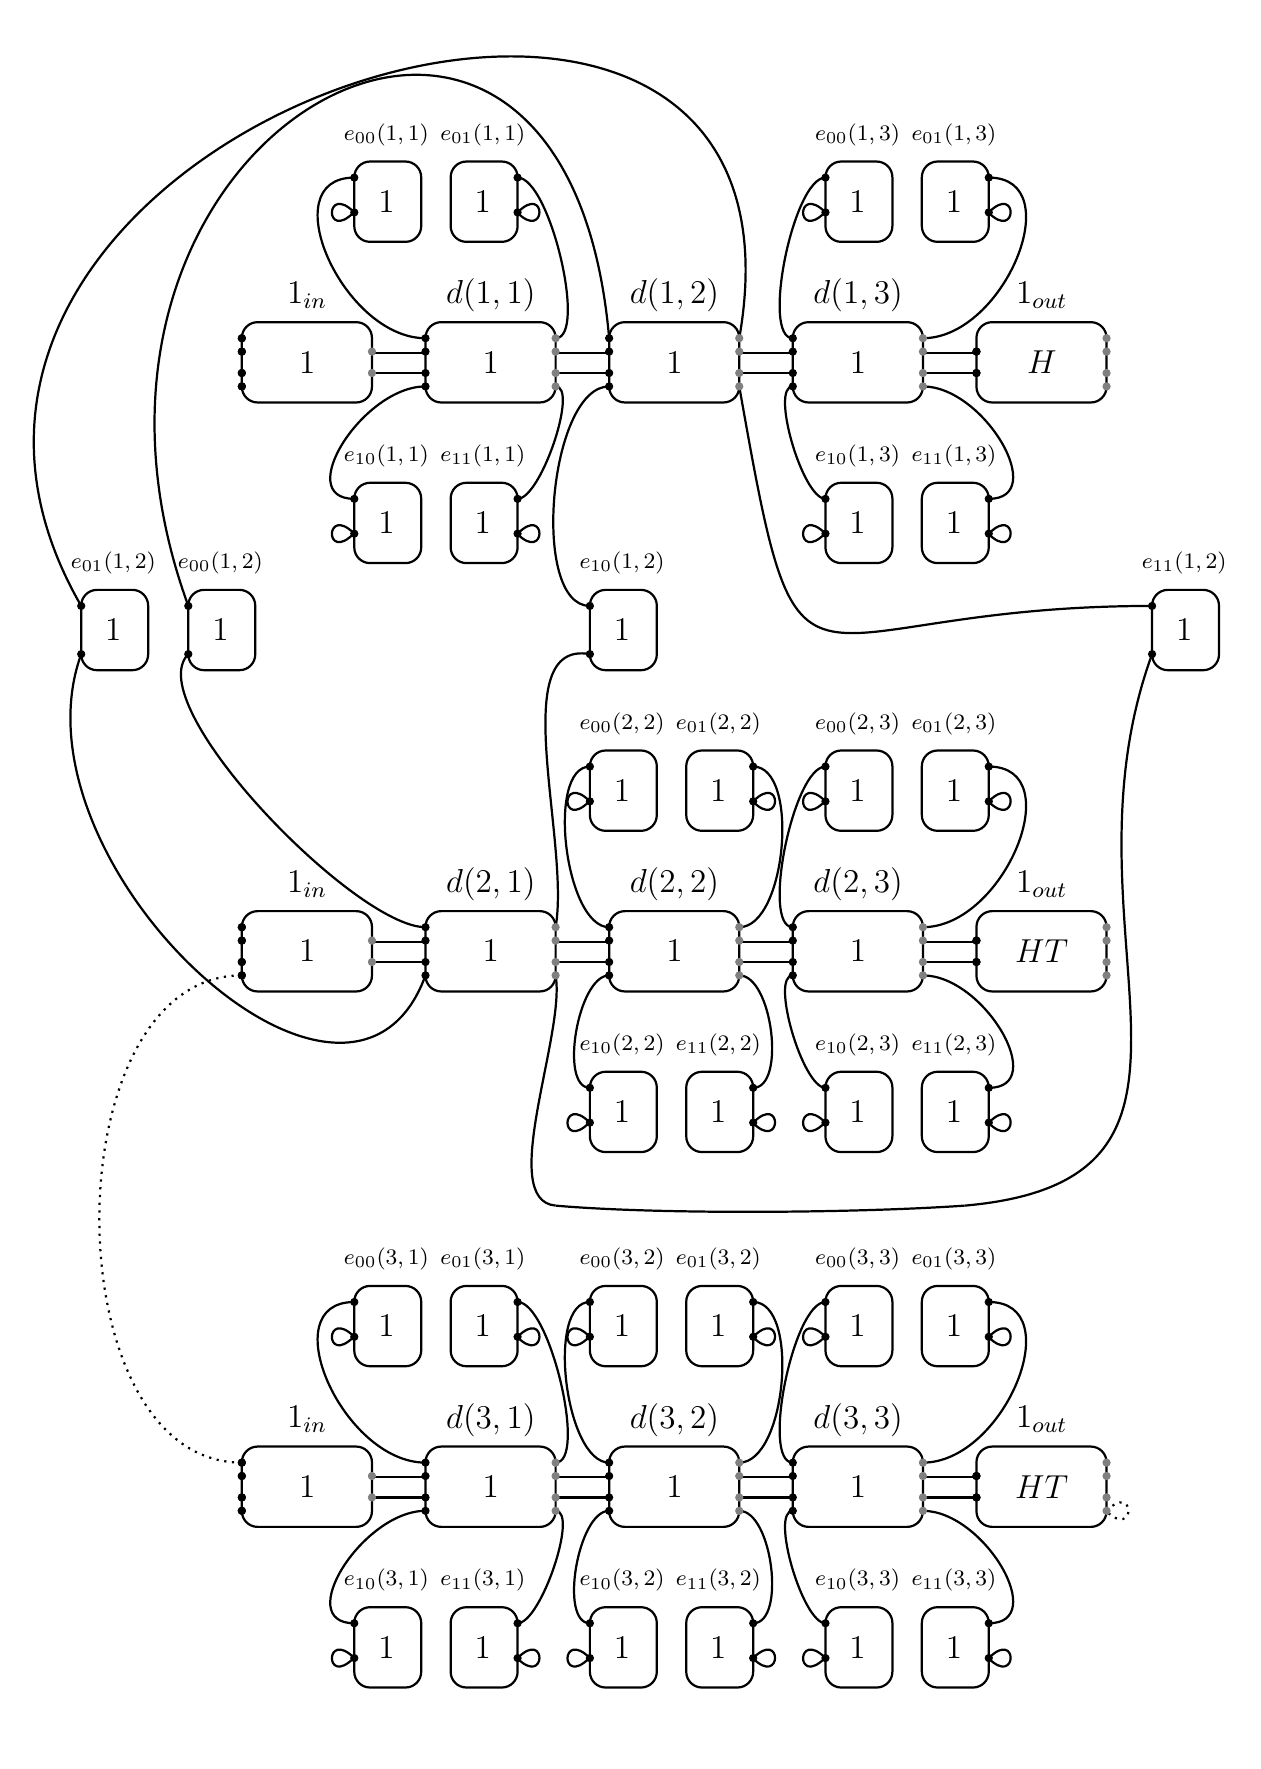
\begin{tikzpicture}[scale=0.68]
\path[use as bounding box](-4,-25) rectangle (18.5,7);
%%%%%%%%%%%%%%%%%%%%%%%%%%%%%%%%% q=1/2 shared elements
\begin{scope}[yshift=-5cm]
%%%%%%%% e00
\foreach \offset/\unitary/\label in
{-1/1/{e_{00}(1,2)}}
{   
\begin{scope}[xshift=\offset cm]       
\draw[rounded corners=2mm,thick] (0,0) rectangle (1.25cm,1.5 cm);  
   \foreach \y in {1.2,.3}
{       \draw[fill=black,draw=black] (0 cm, \y cm) circle (.66mm);
    } 
  \node at (0.6cm, .75cm) {\large{$\unitary$}};   
 \node at (0.6cm, 2cm){\footnotesize{$\label$}};
\end{scope}}
%%%%%%%%%%%%% e10
\foreach \offset/\unitary/\label in
{-3/1/{e_{01}(1,2)}}
{   
\begin{scope}[xshift=\offset cm]       
\draw[rounded corners=2mm,thick] (0,0) rectangle (1.25cm,1.5 cm);  
   \foreach \y in {1.2,.3}
{       \draw[fill=black,draw=black] (0 cm, \y cm) circle (.66mm);
    } 
  \node at (0.6cm, .75cm) {\large{$\unitary$}};   
 \node at (0.6cm, 2cm){\footnotesize{$\label$}};
\end{scope}}
\begin{scope}
%%%%%%%% e01
\foreach \offset/\unitary/\label in
{6.5/1/{e_{10}(1,2)}}
{   
\begin{scope}[xshift=\offset cm]       
\draw[rounded corners=2mm,thick] (0,0) rectangle (1.25cm,1.5 cm);  
   \foreach \y in {1.2,.3}
{       \draw[fill=black,draw=black] (0 cm, \y cm) circle (.66mm);
    } 
  \node at (0.6cm, .75cm) {\large{$\unitary$}};   
 \node at (0.6cm, 2cm){\footnotesize{$\label$}};
\end{scope}}
%%%%%%%%%%%%% e11
\foreach \offset/\unitary/\label in
{17/1/{e_{11}(1,2)}}
{   
\begin{scope}[xshift=\offset cm]       
\draw[rounded corners=2mm,thick] (0,0) rectangle (1.25cm,1.5 cm);  
   \foreach \y in {1.2,.3}
{       \draw[fill=black,draw=black] (0 cm, \y cm) circle (.66mm);
    } 
  \node at (0.6cm, .75cm) {\large{$\unitary$}};   
 \node at (0.6cm, 2cm){\footnotesize{$\label$}};
\end{scope}}
\end{scope}

%%%%%%
% these are the stuff
\draw[thick,looseness = 2.6] (6.86,6.2) to [out = 95, in = 110] (-1,1.2); 
\draw[thick,looseness = 0.5] (3.43,-4.8) to [out = 180, in = 225] (-1,0.3); 
\draw[thick,looseness = 1.2] (3.43,-5.7) to [out = 250, in = 250] (-3,0.3); 
\draw[thick,looseness = 0.7] (6.86,5.3) to [out = 180, in = 180] (6.5,1.2); 
\draw[thick,looseness = 0.8] (5.86,-4.8) to [out = 80, in = 170] (6.5,0.3); 

\draw[thick,looseness = 2] (9.29,5.3) to [out =-80, in = 180] (17,1.2);  
\draw[thick,looseness = 1.3] (13.5,-10) to [out =5, in = 250] (17,0.3);
\draw[thick,looseness = 0.66] (5.86,-10) to [out =-5, in = 184] (13.5,-10);
\draw[thick,looseness = 0.66] (5.86,-5.7) to [out =-80, in = 175] (5.86,-10);
\draw[thick,looseness = 2] (9.29,6.2) to [out =80, in = 120] (-3,1.2); 
\end{scope}

%%%%%%%%%%%%%%%%%%%%%%%%%%%%%%%%% q=1
\begin{scope}
\begin{scope}[yshift=3cm]
% The rectangles above q=1, odd ones
\foreach \offset/\unitary/\label in
{2.1/1/{e_{00}(1,1)},10.9/1/{e_{00}(1,3)}}
{   
\begin{scope}[xshift=\offset cm]       
\draw[rounded corners=2mm,thick] (0,0) rectangle (1.25cm,1.5 cm);  
  \foreach \y in {1.2,.55}
{       \draw[fill=black,draw=black] (0 cm, \y cm) circle (.66mm);
  } 
  \node at (0.6cm, .75cm) {\large{$\unitary$}};   
 \node at (0.6cm, 2cm){\footnotesize{$\label$}};
\draw[thick,looseness = 200] (0,0.55) to [out = 135, in = 225] (-.01,0.55);  
\end{scope}}  
% The rectangles above q=1, even ones
\foreach \offset/\unitary/\label in
{3.9/1/{e_{01}(1,1)},12.7/1/{e_{01}(1,3)}}
{   
\begin{scope}[xshift=\offset cm]       
\draw[rounded corners=2mm,thick] (0,0) rectangle (1.25cm,1.5 cm);  
  \foreach \y in {1.2,.55}
  {       \draw[fill=black,draw=black] (1.25 cm, \y cm) circle (.66mm);
    }
  \node at (0.6cm, .75cm) {\large{$\unitary$}};   
 \node at (0.6cm, 2cm){\footnotesize{$\label$}};
\draw[thick,looseness = 200] (1.25,0.55) to [out = 45, in = -45] (1.24,0.55);  
\end{scope}} 

 
\draw[thick,looseness = 1.2] (3.43,-1.8) to [out = 180, in = 180] (2.1,1.2); 
\draw[thick,looseness = 0.5] (5.86,-1.8) to [out = 0, in = 0] (5.15,1.2); 
\draw[thick,looseness = 0.5] (10.29,-1.8) to [out = 180, in = 180] (10.9,1.2); 
\draw[thick,looseness = 1.2] (12.72,-1.8) to [out = 0, in = 0] (13.95,1.2); 
\end{scope}
\begin{scope}[yshift=-3cm]
% The rectangles below q=1, odd ones
\foreach \offset/\unitary/\label in
{2.1/1/{e_{10}(1,1)},10.9/1/{e_{10}(1,3)}}
{   
\begin{scope}[xshift=\offset cm]       
\draw[rounded corners=2mm,thick] (0,0) rectangle (1.25cm,1.5 cm);  
  \foreach \y in {1.2,.55}
{       \draw[fill=black,draw=black] (0 cm, \y cm) circle (.66mm);
  } 
  \node at (0.6cm, .75cm) {\large{$\unitary$}};   
 \node at (0.6cm, 2cm){\footnotesize{$\label$}};
\draw[thick,looseness = 200] (0,0.55) to [out = 135, in = 225] (-.01,0.55);  
\end{scope}}  

% The rectangles below q=1, even ones
\foreach \offset/\unitary/\label in
{3.9/1/{e_{11}(1,1)},12.7/1/{e_{11}(1,3)}}
{   
\begin{scope}[xshift=\offset cm]       
\draw[rounded corners=2mm,thick] (0,0) rectangle (1.25cm,1.5 cm);  
  \foreach \y in {1.2,.55}
  {       \draw[fill=black,draw=black] (1.25 cm, \y cm) circle (.66mm);
    }
  \node at (0.6cm, .75cm) {\large{$\unitary$}};   
 \node at (0.6cm, 2cm){\footnotesize{$\label$}};
\draw[thick,looseness = 200] (1.25,0.55) to [out = 45, in = -45] (1.24,0.55);  
\end{scope}} 


\draw[thick,looseness = 1.2] (3.43,3.3) to [out = 180, in = 180] (2.1,1.2); 
\draw[thick,looseness = 0.5] (5.86,3.3) to [out = 0, in = 0] (5.15,1.2); 
\draw[thick,looseness = 0.5] (10.29,3.3) to [out = 180, in = 180] (10.9,1.2); 
\draw[thick,looseness = 1.2] (12.72,3.3) to [out = 0, in = 0] (13.95,1.2); 
\end{scope}
  % The connections 
 \foreach \y in {0.925,.55}{  
  \draw[thick] (2.43,\y) -- (3.43,\y);
	\draw[thick] (5.86,\y) -- (6.86,\y);	
	\draw[thick] (9.29,\y) -- (10.29,\y);
	\draw[thick] (12.72,\y) -- (13.72,\y);
}
  % The rectangles 
  

\draw[rounded corners=2mm,thick] (0,0) rectangle (2.43cm,1.5 cm);  
  \foreach \x /\color in {0/black,2.43/gray}
  \foreach \y in {1.2,.95,.55,.3}
  {       \draw[fill=black,draw=black] (0 cm, \y cm) circle (.66mm);
  }
  \foreach \y in {.95,.55}
  {       \draw[fill=gray,draw=gray] (2.43 cm, \y cm) circle (.66mm);
  } 
  \node at (1.22cm, .75cm) {\large{$1$}};   
 \node at (1.22cm, 2cm){\large{$1_{\text{in}}$}}; 
 
\begin{scope}[xshift = 13.72 cm] 
 \draw[rounded corners=2mm,thick] (0,0) rectangle (2.43cm,1.5 cm);  
  \foreach \x /\color in {0/black,2.43/gray}
  \foreach \y in {.95,.55}
  {       \draw[fill=black,draw=black] (0 cm, \y cm) circle (.66mm);
  }
  \foreach \y in {1.2,.95,.55,.3}
  {       \draw[fill=gray,draw=gray] (2.43 cm, \y cm) circle (.66mm);
  } 
  \node at (1.22cm, .75cm) {\large{$H$}};   
 \node at (1.22cm, 2cm){\large{$1_{\text{out}}$}};   
\end{scope}

  
 \foreach \offset/\unitary/\label in {3.43/1/{d(1,1)},6.86/1/{d(1,2)},10.29/1/{d(1,3)}}
{   
\begin{scope}[xshift=\offset cm]       
\draw[rounded corners=2mm,thick] (0,0) rectangle (2.43cm,1.5 cm);  
  \foreach \x /\color in {0/black,2.43/gray}
{     \foreach \y in {1.2,.95,.55,.3}
{       \draw[fill=\color,draw=\color] (\x cm, \y cm) circle (.66mm);
    }} 
  \node at (1.22cm, .75cm) {\large{$\unitary$}};   
 \node at (1.22cm, 2cm){\large{$\label$}};   
\end{scope}}  
\end{scope}

%%%%%%%%%%%%%%%%%%%%%%%%%%%%%%%%% q=2
\begin{scope}[yshift=-11cm]
\begin{scope}[yshift=3cm]



% The rectangles above q=2, odd ones
\foreach \offset/\unitary/\label in
{6.5/1/{e_{00}(2,2)},10.9/1/{e_{00}(2,3)}}
{   
\begin{scope}[xshift=\offset cm]       
\draw[rounded corners=2mm,thick] (0,0) rectangle (1.25cm,1.5 cm);  
  \foreach \y in {1.2,.55}
{       \draw[fill=black,draw=black] (0 cm, \y cm) circle (.66mm);
  } 
  \node at (0.6cm, .75cm) {\large{$\unitary$}};   
 \node at (0.6cm, 2cm){\footnotesize{$\label$}};
\draw[thick,looseness = 200] (0,0.55) to [out = 135, in = 225] (-.01,0.55);  
\end{scope}}   
\end{scope}
\begin{scope}[yshift=3cm]
% The rectangles above q=2, even ones
\draw[thick,looseness = 0.7] (6.86,-1.8) to [out = 180, in = 180] (6.5,1.2); 
\draw[thick,looseness = 0.75] (9.29,-1.8) to [out = 0, in = 0] (9.55,1.2); 
\draw[thick,looseness = 0.5] (10.29,-1.8) to [out = 180, in = 180] (10.9,1.2); 
\draw[thick,looseness = 1.2] (12.72,-1.8) to [out = 0, in = 0] (13.95,1.2); 
\foreach \offset/\unitary/\label in
{8.3/1/{e_{01}(2,2)},12.7/1/{e_{01}(2,3)}}
{   
\begin{scope}[xshift=\offset cm]       
\draw[rounded corners=2mm,thick] (0,0) rectangle (1.25cm,1.5 cm);  
  \foreach \y in {1.2,.55}
  {       \draw[fill=black,draw=black] (1.25 cm, \y cm) circle (.66mm);
    }
  \node at (0.6cm, .75cm) {\large{$\unitary$}};   
 \node at (0.6cm, 2cm){\footnotesize{$\label$}};
\draw[thick,looseness = 200] (1.25,0.55) to [out = 45, in = -45] (1.24,0.55);  
\end{scope}}   
\end{scope}
\begin{scope}[yshift=-3cm]
% The rectangles below q=2, odd ones
\foreach \offset/\unitary/\label in
{6.5/1/{e_{10}(2,2)},10.9/1/{e_{10}(2,3)}}
{   
\begin{scope}[xshift=\offset cm]       
\draw[rounded corners=2mm,thick] (0,0) rectangle (1.25cm,1.5 cm);  
  \foreach \y in {1.2,.55}
{       \draw[fill=black,draw=black] (0 cm, \y cm) circle (.66mm);
  } 
  \node at (0.6cm, .75cm) {\large{$\unitary$}};   
 \node at (0.6cm, 2cm){\footnotesize{$\label$}};
\draw[thick,looseness = 200] (0,0.55) to [out = 135, in = 225] (-.01,0.55);  
\end{scope}}  
\end{scope}
\begin{scope}[yshift=-3cm]
% The rectangles below q=2, even ones
\foreach \offset/\unitary/\label in
{8.3/1/{e_{11}(2,2)},12.7/1/{e_{11}(2,3)}}
{   
\begin{scope}[xshift=\offset cm]       
\draw[rounded corners=2mm,thick] (0,0) rectangle (1.25cm,1.5 cm);  
  \foreach \y in {1.2,.55}
  {       \draw[fill=black,draw=black] (1.25 cm, \y cm) circle (.66mm);
    }
  \node at (0.6cm, .75cm) {\large{$\unitary$}};   
 \node at (0.6cm, 2cm){\footnotesize{$\label$}};
\draw[thick,looseness = 200] (1.25,0.55) to [out = 45, in = -45] (1.24,0.55);  
\end{scope}}   
\draw[thick,looseness = 0.7] (6.86,3.3) to [out = 180, in = 180] (6.5,1.2); 
\draw[thick,looseness = 0.75] (9.29,3.3) to [out = 0, in = 0] (9.55,1.2); 
\draw[thick,looseness = 0.5] (10.29,3.3) to [out = 180, in = 180] (10.9,1.2); 
\draw[thick,looseness = 1.2] (12.72,3.3) to [out = 0, in = 0] (13.95,1.2); 
\end{scope}
  % The connections 
 \foreach \y in {0.925,.55}{  
  \draw[thick] (2.43,\y) -- (3.43,\y);
	\draw[thick] (5.86,\y) -- (6.86,\y);	
	\draw[thick] (9.29,\y) -- (10.29,\y);
	\draw[thick] (12.72,\y) -- (13.72,\y);
}
  % The rectangles 
  \draw[rounded corners=2mm,thick] (0,0) rectangle (2.43cm,1.5 cm);  
  \foreach \x /\color in {0/black,2.43/gray}
  \foreach \y in {1.2,.95,.55,.3}
  {       \draw[fill=black,draw=black] (0 cm, \y cm) circle (.66mm);
  }
  \foreach \y in {.95,.55}
  {       \draw[fill=gray,draw=gray] (2.43 cm, \y cm) circle (.66mm);
  } 
  \node at (1.22cm, .75cm) {\large{$1$}};   
 \node at (1.22cm, 2cm){\large{$1_{\text{in}}$}}; 
 
\begin{scope}[xshift = 13.72 cm] 
 \draw[rounded corners=2mm,thick] (0,0) rectangle (2.43cm,1.5 cm);  
  \foreach \x /\color in {0/black,2.43/gray}
  \foreach \y in {.95,.55}
  {       \draw[fill=black,draw=black] (0 cm, \y cm) circle (.66mm);
  }
  \foreach \y in {1.2,.95,.55,.3}
  {       \draw[fill=gray,draw=gray] (2.43 cm, \y cm) circle (.66mm);
  } 
  \node at (1.22cm, .75cm) {\large{$HT$}};   
 \node at (1.22cm, 2cm){\large{$1_{\text{out}}$}};   
\end{scope}
  
 \foreach \offset/\unitary/\label in {3.43/1/{d(2,1)},6.86/1/{d(2,2)},10.29/1/{d(2,3)}}
{   
\begin{scope}[xshift=\offset cm]       
\draw[rounded corners=2mm,thick] (0,0) rectangle (2.43cm,1.5 cm);  
  \foreach \x /\color in {0/black,2.43/gray}
{     \foreach \y in {1.2,.95,.55,.3}
{       \draw[fill=\color,draw=\color] (\x cm, \y cm) circle (.66mm);
    }} 
  \node at (1.22cm, .75cm) {\large{$\unitary$}};   
 \node at (1.22cm, 2cm){\large{$\label$}};   
\end{scope}}
\end{scope}

%%%%%%%%%%%%%%%%%%%%%%%%%%%%%%%%% q=3
\begin{scope}[yshift=-21cm]
%%%%%%%%%%%%% Edge and self-loop from G
\draw[thick,dotted,looseness = 200] (16.15,0.3) to [out = 45, in = -45] (16.14,0.3); 
\draw[thick,dotted,looseness = 1] (0,1.2) to [out =180, in = 180] (0,10.3);

\begin{scope}[yshift=3cm]
% The rectangles above q=3, odd ones
\foreach \offset/\unitary/\label in
{2.1/1/{e_{00}(3,1)},6.5/1/{e_{00}(3,2)},10.9/1/{e_{00}(3,3)}}
{   
\begin{scope}[xshift=\offset cm]       
\draw[rounded corners=2mm,thick] (0,0) rectangle (1.25cm,1.5 cm);  
  \foreach \y in {1.2,.55}
{       \draw[fill=black,draw=black] (0 cm, \y cm) circle (.66mm);
  } 
  \node at (0.6cm, .75cm) {\large{$\unitary$}};   
 \node at (0.6cm, 2cm){\footnotesize{$\label$}};
\draw[thick,looseness = 200] (0,0.55) to [out = 135, in = 225] (-.01,0.55);  
\end{scope}} 
\end{scope}
\begin{scope}[yshift=3cm]
% The rectangles above q=3, even ones
\foreach \offset/\unitary/\label in
{3.9/1/{e_{01}(3,1)},8.3/1/{e_{01}(3,2)},12.7/1/{e_{01}(3,3)}}
{   
\begin{scope}[xshift=\offset cm]       
\draw[rounded corners=2mm,thick] (0,0) rectangle (1.25cm,1.5 cm);  
  \foreach \y in {1.2,.55}
  {       \draw[fill=black,draw=black] (1.25 cm, \y cm) circle (.66mm);
    }
  \node at (0.6cm, .75cm) {\large{$\unitary$}};   
 \node at (0.6cm, 2cm){\footnotesize{$\label$}};
\draw[thick,looseness = 200] (1.25,0.55) to [out = 45, in = -45] (1.24,0.55);  
\end{scope}}  
\draw[thick,looseness = 1.2] (3.43,-1.8) to [out = 180, in = 180] (2.1,1.2); 
\draw[thick,looseness = 0.5] (5.86,-1.8) to [out = 0, in = 0] (5.15,1.2); 
\draw[thick,looseness = 0.7] (6.86,-1.8) to [out = 180, in = 180] (6.5,1.2); 
\draw[thick,looseness = 0.75] (9.29,-1.8) to [out = 0, in = 0] (9.55,1.2); 
\draw[thick,looseness = 0.5] (10.29,-1.8) to [out = 180, in = 180] (10.9,1.2); 
\draw[thick,looseness = 1.2] (12.72,-1.8) to [out = 0, in = 0] (13.95,1.2); 
\end{scope}
\begin{scope}[yshift=-3cm]
% The rectangles below q=3, odd ones
\foreach \offset/\unitary/\label in
{2.1/1/{e_{10}(3,1)},6.5/1/{e_{10}(3,2)},10.9/1/{e_{10}(3,3)}}
{   
\begin{scope}[xshift=\offset cm]       
\draw[rounded corners=2mm,thick] (0,0) rectangle (1.25cm,1.5 cm);  
  \foreach \y in {1.2,.55}
{       \draw[fill=black,draw=black] (0 cm, \y cm) circle (.66mm);
  } 
  \node at (0.6cm, .75cm) {\large{$\unitary$}};   
 \node at (0.6cm, 2cm){\footnotesize{$\label$}};
\draw[thick,looseness = 200] (0,0.55) to [out = 135, in = 225] (-.01,0.55);  
\end{scope}}   
\end{scope}
\begin{scope}[yshift=-3cm]
% The rectangles below q=3, even ones
\foreach \offset/\unitary/\label in
{3.9/1/{e_{11}(3,1)},8.3/1/{e_{11}(3,2)},12.7/1/{e_{11}(3,3)}}
{   
\begin{scope}[xshift=\offset cm]       
\draw[rounded corners=2mm,thick] (0,0) rectangle (1.25cm,1.5 cm);  
  \foreach \y in {1.2,.55}
  {       \draw[fill=black,draw=black] (1.25 cm, \y cm) circle (.66mm);
    }
  \node at (0.6cm, .75cm) {\large{$\unitary$}};   
 \node at (0.6cm, 2cm){\footnotesize{$\label$}};
\draw[thick,looseness = 200] (1.25,0.55) to [out = 45, in = -45] (1.24,0.55);  
\end{scope}}     
\draw[thick,looseness = 1.2] (3.43,3.3) to [out = 180, in = 180] (2.1,1.2); 
\draw[thick,looseness = 0.5] (5.86,3.3) to [out = 0, in = 0] (5.15,1.2); 
\draw[thick,looseness = 0.7] (6.86,3.3) to [out = 180, in = 180] (6.5,1.2); 
\draw[thick,looseness = 0.75] (9.29,3.3) to [out = 0, in = 0] (9.55,1.2); 
\draw[thick,looseness = 0.5] (10.29,3.3) to [out = 180, in = 180] (10.9,1.2); 
\draw[thick,looseness = 1.2] (12.72,3.3) to [out = 0, in = 0] (13.95,1.2); 
\end{scope}
  % The connections 
 \foreach \y in {0.925,.55}{  
  \draw[thick] (2.43,\y) -- (3.43,\y);
	\draw[thick] (5.86,\y) -- (6.86,\y);	
	\draw[thick] (9.29,\y) -- (10.29,\y);
	\draw[thick] (12.72,\y) -- (13.72,\y);
}
  % The rectangles 
    \draw[rounded corners=2mm,thick] (0,0) rectangle (2.43cm,1.5 cm);  
  \foreach \x /\color in {0/black,2.43/gray}
  \foreach \y in {1.2,.95,.55,.3}
  {       \draw[fill=black,draw=black] (0 cm, \y cm) circle (.66mm);
  }
  \foreach \y in {.95,.55}
  {       \draw[fill=gray,draw=gray] (2.43 cm, \y cm) circle (.66mm);
  } 
  \node at (1.22cm, .75cm) {\large{$1$}};   
 \node at (1.22cm, 2cm){\large{$1_{\text{in}}$}}; 
 
\begin{scope}[xshift = 13.72 cm] 
 \draw[rounded corners=2mm,thick] (0,0) rectangle (2.43cm,1.5 cm);  
  \foreach \x /\color in {0/black,2.43/gray}
  \foreach \y in {.95,.55}
  {       \draw[fill=black,draw=black] (0 cm, \y cm) circle (.66mm);
  }
  \foreach \y in {1.2,.95,.55,.3}
  {       \draw[fill=gray,draw=gray] (2.43 cm, \y cm) circle (.66mm);
  } 
  \node at (1.22cm, .75cm) {\large{$HT$}};   
 \node at (1.22cm, 2cm){\large{$1_{\text{out}}$}};   
\end{scope}
  
 \foreach \offset/\unitary/\label in {3.43/1/{d(3,1)},6.86/1/{d(3,2)},10.29/1/{d(3,3)}}
{   
\begin{scope}[xshift=\offset cm]       
\draw[rounded corners=2mm,thick] (0,0) rectangle (2.43cm,1.5 cm);  
  \foreach \x /\color in {0/black,2.43/gray}
{     \foreach \y in {1.2,.95,.55,.3}
{       \draw[fill=\color,draw=\color] (\x cm, \y cm) circle (.66mm);
    }} 
  \node at (1.22cm, .75cm) {\large{$\unitary$}};   
 \node at (1.22cm, 2cm){\large{$\label$}};   
\end{scope}}  
\end{scope}
\end{tikzpicture}